\begin{frame}{Equilibria in 2-Player Signaling Games}
  \begin{itemize}
    \item So far we have covered the general concepts of incomplete information.
    \item We saw how \alert{adverse selection} can arise 
    in games with many players.
    \item But now we will solve for equilibria 
    in the case of a simpler 2-player game.
  \end{itemize} 
\end{frame}

% - - - - - - - - - - - - - - - - - - - - - - - - - - - - - - - - - - - - - - - 

\begin{frame}{Semiseparating Equilibria}
  \begin{itemize}
    \item We saw \alert{Pooling Equilibria} 
    in which all types take the same action
    \begin{itemize}
      \item aka \textit{'babbling  equilibria'}
    \end{itemize}
    \item And we also saw \alert{Separating Equilibria}
    in which different types take \textit{completely different} actions
    \begin{itemize}
      \item sometimes called \textit{'cheap talk equilibria'} 
    \end{itemize}
  \end{itemize}
\end{frame}

% - - - - - - - - - - - - - - - - - - - - - - - - - - - - - - - - - - - - - - - 

\begin{frame}{Market Entry Game}
  \begin{itemize}
    \item \textbf{Players:} competing auto manufacturers:
    \alert{Tudor} and \alert{Fordor}
    \item \alert{Tudor} is a current monopolist in the auto industry 
    \item \alert{Fordor} is a potential entrant in the market 
    \item \alert{Tudor} has \textbf{private information} 
    on how tough they will be able to compete against a \alert{Fordor} entrant. 
  \end{itemize}
\end{frame}

% - - - - - - - - - - - - - - - - - - - - - - - - - - - - - - - - - - - - - - - 

\begin{frame}{Market Entry Game}
  \textbf{Sequential Game}
  \begin{itemize}
    \item \textbf{Stage 1:} Tudor sets price $\in \{ low,~high \}$ 
    \item \textbf{Stage 2:} Fordor makes entry decision $\in \{ in,~out \}$
  \end{itemize} 
  \textbf{Payouts:}
  \begin{itemize}
    \item Profits for each firm are market price - production costs
    \begin{itemize}
      \item \textbf{Market Demand:} $P = 25 - Q$ 
    \end{itemize}
  \end{itemize}
\end{frame}

% - - - - - - - - - - - - - - - - - - - - - - - - - - - - - - - - - - - - - - - 

\begin{frame}{Market Entry Game}
  \textbf{Costs:}
  \begin{itemize}
    \item \alert{Fordor}'s upfront cost of entry: 40 
    \item \alert{Fordor}'s per-unit cost: 10
    \item \alert{Tudor}'s costs:
    \begin{itemize}
      \item If \textbf{high-cost}: 15
      \item If \textbf{low-cost}:  5
    \end{itemize}
  \end{itemize}
\end{frame}

% - - - - - - - - - - - - - - - - - - - - - - - - - - - - - - - - - - - - - - - 

\begin{frame}{Market Entry Game}
  \textbf{Payouts:} 
  \begin{itemize}
    \item \underline{If Tudor is high-cost:} 
    \begin{itemize}
      \item and \underline{Fordor stays out:} 
      $\Pi_{T1} = 5 * (20-15) = 25$ and $\Pi_{T2} = 25$, 
      $\Pi_{F} = 0$
      \item and \underline{Fordor enters:}
      $\Pi_{T} = 25 + 3$,
      $\Pi_{F} = 45 $ - startup cost of 40 
    \end{itemize}
    \item \underline{If Tudor is low-cost:}
    \begin{itemize}
      \item and \underline{Fordor stays out:}
      $\Pi_{T1} = 100$ and $\Pi_{T2} = 100$, 
      $\Pi_{F} = 0$
      \item \underline{Fordor enters:}
      $\Pi_{T} = 100 + 69$,
      $\Pi_{F} = 11$ - startup cost of 40 
    \end{itemize}
  \end{itemize}
\end{frame}
% - - - - - - - - - - - - - - - - - - - - - - - - - - - - - - - - - - - - - - - 

\begin{frame}{Market Entry - Extensive Form Game}
  \begin{center}
    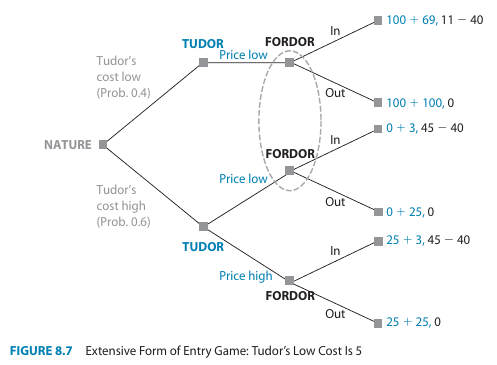
\includegraphics[width=.9\textwidth]{figures/Fig87.png} 
  \end{center} 
\end{frame}

% - - - - - - - - - - - - - - - - - - - - - - - - - - - - - - - - - - - - - - - 

\begin{frame}{Market Entry Game}
  \textbf{Signaling Strategies}
  \begin{itemize}
    \item Tudor might use its price as a \alert{signal} of its cost.
    \item A \textit{low-cost} firm would charge a lower price, 
    so Tudor might hope to keep its price low to show Fordor that they 
    are a low-cost firm and therefore more difficult to fight.
    \item However, Tudor might also try to \textbf{bluff} Fordor 
    into staying out.
  \end{itemize}
\end{frame}

% - - - - - - - - - - - - - - - - - - - - - - - - - - - - - - - - - - - - - - - 

\begin{frame}{Market Entry Game - Separating Equilibrium}
  \textbf{Checking for Separating Equilibrium:} 
  \begin{enumerate}
    \item \textbf{Step 1:} Prune strategies using rollback: 
    \begin{itemize}
      \item What should \alert{Fordor} do if they see a \textbf{high price}?
    \end{itemize}
  \end{enumerate}
  \begin{center}
    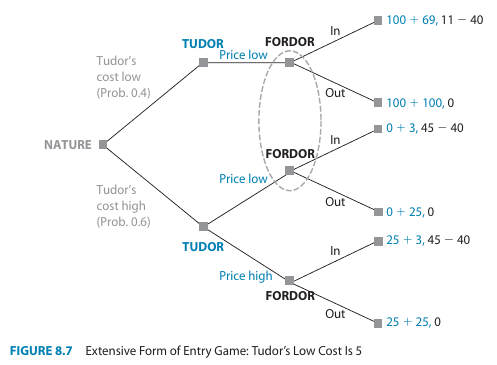
\includegraphics[width=.7\textwidth]{figures/Fig87.png} 
  \end{center} 
\end{frame}

% - - - - - - - - - - - - - - - - - - - - - - - - - - - - - - - - - - - - - - - 

\begin{frame}{Market Entry Game - Separating Equilibrium}
  \textbf{Checking for Separating Equilibrium:} \\ 
  \begin{itemize}
    \item How many Strategies does each player have? 
    \begin{itemize}
      \item (After pruning \textit{Out if Price High} for \alert{Fordor}) 
    \end{itemize}
  \end{itemize}
\end{frame}

% - - - - - - - - - - - - - - - - - - - - - - - - - - - - - - - - - - - - - - - 

\begin{frame}{Market Entry Game - Separating Equilibrium}
  \textbf{Checking for Separating Equilibrium:} \\ 
  \textbf{Step 2:} Represent game in \textit{Strategic Form:}
  \begin{center}
    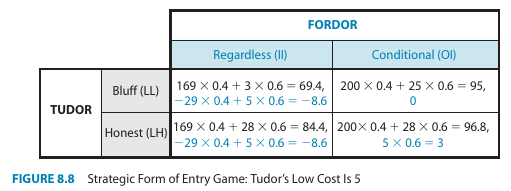
\includegraphics[width =.9\textwidth]{figures/Fig88.png} 
  \end{center}
\end{frame}

% - - - - - - - - - - - - - - - - - - - - - - - - - - - - - - - - - - - - - - - 

\begin{frame}{Market Entry Game - Separating Equilibrium}
  \textbf{Checking for Separating Equilibrium:} \\ 
  \textbf{Step 3:} Look for NE in the \textit{Strategic Form}
  \begin{center}
    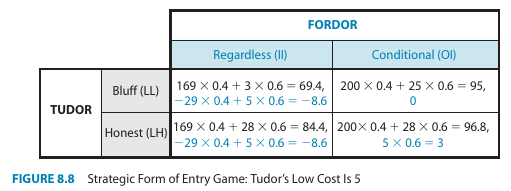
\includegraphics[width =.9\textwidth]{figures/Fig88.png} 
  \end{center}
\end{frame}

% - - - - - - - - - - - - - - - - - - - - - - - - - - - - - - - - - - - - - - - 

\begin{frame}{Market Entry Game - Separating Equilibrium}
  \textbf{Checking for Separating Equilibrium:} \\ 
  \begin{itemize}
    \item So when Tudor's Low Cost is 5, 
    the Nash Equilibrium is (Honest, Conditional)
    \item This is a \textit{Separating} equilibrium,
    because the Tudor's action of \textit{Price High} or \textit{Price Low}
    completely reveals their type to Fordor.
  \end{itemize}
\end{frame}

% - - - - - - - - - - - - - - - - - - - - - - - - - - - - - - - - - - - - - - - 

\begin{frame}{Market Entry Game}
  Is it guaranteed that this game will \textit{always} 
  result in complete separation of types?
  \begin{itemize}
    \item What if we change the Tudor's Low Cost to 10 instead of 5? 
  \end{itemize}
\end{frame}

% - - - - - - - - - - - - - - - - - - - - - - - - - - - - - - - - - - - - - - - 

\begin{frame}{Market Entry Game - Pooling Equilibrium}
  Can you prune any strategies?
  \begin{center}
    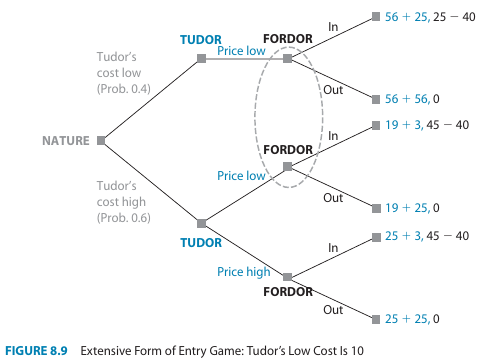
\includegraphics[width=.9\textwidth]{figures/Fig89.png}
  \end{center}
\end{frame}

% - - - - - - - - - - - - - - - - - - - - - - - - - - - - - - - - - - - - - - - 

\begin{frame}{Market Entry Game - Pooling Equilibrium}
  Now what is the Nash Equilibrium of this game?
  \begin{center}
    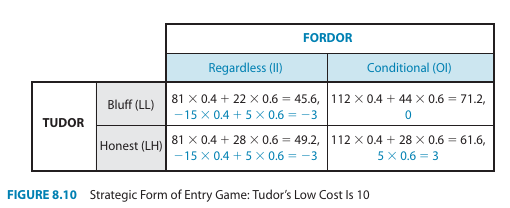
\includegraphics[width=.9\textwidth]{figures/Fig810.png}
  \end{center}
\end{frame}

% - - - - - - - - - - - - - - - - - - - - - - - - - - - - - - - - - - - - - - - 

\begin{frame}{Market Entry Game - Pooling Equilibrium}
  \begin{itemize}
    \item So when Tudor's Low Cost is \alert{10}, 
    the Nash Equilibrium is (\alert{Bluff}, Conditional)
    \item This is a \textit{Pooling} equilibrium,
    because Tudor always takes the same action of \textit{Price Low}. \\ 
    This gives Fordor no signal of their type, 
    but Fordor still doesn't have any incentive to change their strategy.
  \end{itemize}
\end{frame}

% - - - - - - - - - - - - - - - - - - - - - - - - - - - - - - - - - - - - - - - 

\begin{frame}{Market Entry Game}
  \begin{itemize}
    \item So far, we found that depending on the relative difference
    between a \textit{low-cost} Tudor and a \textit{high-cost} Tudor,
    there may either be a \textbf{Pooling} or \textbf{Separating} equilibrium.
    \item But there might also be an equilibrium somewhere in between: 
    where there is \textit{partial} sorting of types
    \item We call this type of equilibrium \textbf{Semiseparating}
  \end{itemize}
\end{frame}

% - - - - - - - - - - - - - - - - - - - - - - - - - - - - - - - - - - - - - - - 

\begin{frame}{Market Entry Game - Semiseparating}
  Now let's change the original probability that a Tudor is low cost
  from .4 to .1
  \begin{itemize}
    \item (But keep all of the payoffs the same as in the last case) 
  \end{itemize}
\end{frame}

% - - - - - - - - - - - - - - - - - - - - - - - - - - - - - - - - - - - - - - - 

\begin{frame}{Market Entry Game - Semiseparating}
  Can you find a Nash Equilibrium with the new expected utilities? 
  \begin{center}
    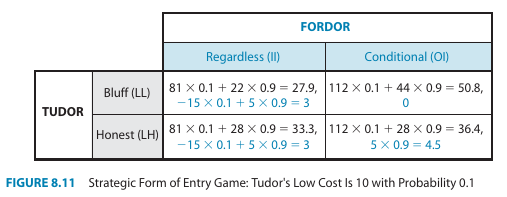
\includegraphics[width=1.0\textwidth]{figures/Fig811.png} 
  \end{center}
\end{frame}

% - - - - - - - - - - - - - - - - - - - - - - - - - - - - - - - - - - - - - - - 

\begin{frame}{Market Entry Game - Semiseparating}
  \textbf{Looking for Mixed Strategy Nash Equilibrium} 
  \begin{itemize}
    \item Suppose \alert{Tudor} plays Bluff with probability $p$,
    Honest with $1-p$ 
    \item When will \alert{Fordor} play a mixed strategy?
  \end{itemize}
\end{frame}

% - - - - - - - - - - - - - - - - - - - - - - - - - - - - - - - - - - - - - - - 

\begin{frame}[plain]{}
  
\end{frame}

% - - - - - - - - - - - - - - - - - - - - - - - - - - - - - - - - - - - - - - - 

\begin{frame}{Market Entry Game - Semiseparating}
  \textbf{Looking for Mixed Strategy Nash Equilibrium} 
  \begin{itemize}
    \item Suppose \alert{Fordor} plays Regardless with probability $q$,
    Conditional with $1-q$ 
    \item When will \alert{Tudor} play a mixed strategy?
  \end{itemize}
\end{frame}

% - - - - - - - - - - - - - - - - - - - - - - - - - - - - - - - - - - - - - - - 

\begin{frame}[plain]{}
  
\end{frame}

% - - - - - - - - - - - - - - - - - - - - - - - - - - - - - - - - - - - - - - - 

\begin{frame}{Market Entry Game - Semiseparating}
  \begin{itemize}
  \item So this version of the game has the MSNE:\\ 
  $\{$ (1/3 Bluff, 2/3 Honest), (16/22 Regardless, 6/22 Conditional) $\}$
  \begin{itemize}
    \item In this equilibrium, instead of \textit{complete separation}  
    or \textit{complete pooling}, 
    we have \alert{\textit{semiseparating}}
    \item A high price conveys full information to Fordor, 
    but a low price could mean that the Tudor is \textit{either} 
    a \textbf{low-price} \textit{or} a \textbf{high-price} type.
  \end{itemize}
  \end{itemize}
\end{frame}

% - - - - - - - - - - - - - - - - - - - - - - - - - - - - - - - - - - - - - - - 

\begin{frame}{Market Entry Game - Semiseparating}
  \textbf{Bayes' Rule} 
  \begin{center}
    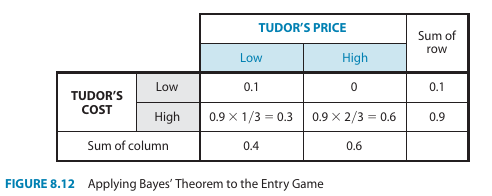
\includegraphics[width=.9\textwidth]{figures/Fig812.png} 
  \end{center}
\end{frame}
